\section{Vérification de la complexité}
\begin{enumerate}[(a)]
  \item \q{Ecrire une fonction }\il{test_tri(n)}\q{ qui :}
        \begin{itemize}
          \item \q{Enregistre dans }\il{Tab}\q{ un tableau de $n$ nombre
                  aléatoires compris entre $0$ et $n$ avec la fonction }
                \il{randint}\q{ du module }\il{numpy.random}
          \item \q{Affiche les 6 premiers termes et les 6 derniers termes de}
                \il{Tab}
          \item \q{Trie }\il{Tab}\q{et donne la durée du tri en secondes}
          \item \q{Affiche les 6 premiers termes et les 6 derniers termes de}
                \il{Tab}\q{ trié}
          \item \q{Retourne la durée du tri}
        \end{itemize}
        \q{Avec cette fonction calculer la durée du tri pour $n\in\{10; 100;
            200; 500; 1500\}$ et vérifier que la durée du tri est
          proportionnelle à $n^2$}


        \bigskip


        Je commence par rajouter deux méthodes à la classe \il{Liste} :
        \begin{dinglist}{111}
          \item \il{generateRadomList} qui génère une liste de n entiers
          aléatoires
          \item \il{time} qui génère et trie des listes de taille allant de $1$
          à $n$, enregistre le temps, et le trace en fonction de $n^2$ si le
          paramètre \il{show} est passé à \il{True}.
        \end{dinglist}
        \bigskip
        \ul{Remarque :} Je n'ai pas affiché les 6 premiers et derniers termes,
        mais il suffirait de rajouter les fonctions :
        \begin{itemize}
          \item \il{print(self.A[:6])} pour afficher les 6 premiers
          \item \il{print(self.A[-6:])} pour les 6 derniers
        \end{itemize}

        \bigskip

        Ensuite, dans \il{main.py} j'exécute la fonction \il{time} sur l'objet
        \il{A}

        \ul{Remarque :} Mon programme teste $n$ listes et non pas 5 comme demandé.
        \newpage
        \codeFromFileT{ressources/liste.py}{section-04/qa-1.py}
        \codeFromFileT{ressources/liste.py}{section-04/qa-2.py}
        \begin{center}
          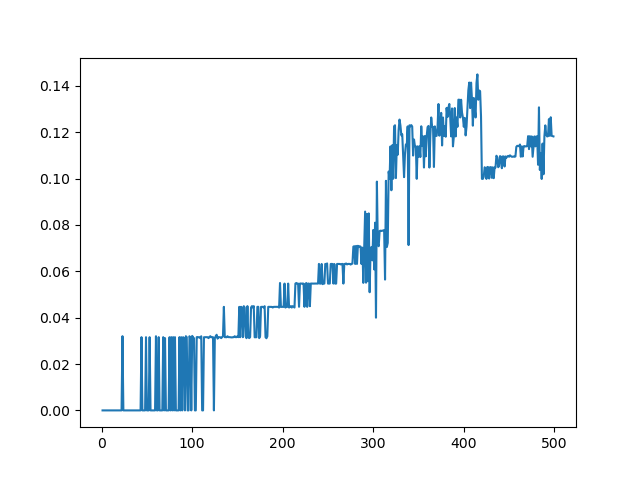
\includegraphics[scale=0.5]{section-04/qa-3.png}
        \end{center}


        On a une mesure très bruitée, mais qui a plutôt tendance à être une
        droite, ce qui prouverait la complexité quadratique.

\end{enumerate}
